% ============================================================
% BAB 3 - KONTEKS OPERASIONAL DAN ARSITEKTUR
% ============================================================

\subsection{Architectural Overview}

Aplikasi menggunakan arsitektur \textbf{monorepo dua-tier} dengan pemisahan
\textit{frontend} dan \textit{backend} yang di-\textit{deploy} secara independen.
\textit{Backend} menggunakan pola modular berbasis domain (\texttt{src/modules/})
dengan \textit{middleware} terpusat untuk auth, validasi, dan \textit{error
handling}. \textit{Frontend} menggunakan App Router Next.js dengan komponen
shadcn/ui dan \textit{state management} Zustand.

\begin{longtable}{|L{3.5cm}|L{5cm}|L{6.5cm}|}
    \caption{Lapisan Arsitektur Sistem PasarKita}
    \label{tab:arsitektur} \\
    \hline
    \textbf{Lapisan} & \textbf{Artefak Utama} & \textbf{Tanggung Jawab} \\
    \hline
    \endfirsthead
    \hline
    \textbf{Lapisan} & \textbf{Artefak Utama} & \textbf{Tanggung Jawab} \\
    \hline
    \endhead
    \hline
    \endfoot
    Frontend: Routing
        & \texttt{frontend/app/} (App Router)
        & Mengarahkan halaman ke komponen React berdasarkan URL. \\
    \hline
    Frontend: UI Components
        & \texttt{frontend/components/}
        & Menyajikan halaman \textit{buyer} (katalog, \textit{cart},
          \textit{checkout}, \textit{order}), \textit{seller}
          (\textit{dashboard}, CRUD produk), dan admin
          (\textit{analytics}, manajemen \textit{user}). \\
    \hline
    Frontend: State
        & \texttt{frontend/store/} (Zustand)
        & Mengelola auth \textit{state} (\textit{user}, token) dan \textit{cart
          state} (\textit{items}, \textit{quantity}) secara \textit{client-side}. \\
    \hline
    Frontend: API Client
        & \texttt{frontend/lib/}
        & \textit{Wrapper} Axios/fetch ke \textit{backend} API dengan \textit{token
          injection} dari Zustand auth \textit{store}. \\
    \hline
    Backend: Entry Point
        & \texttt{backend/api/index.js}
        & \textit{Serverless entry point}; \textit{mounting} semua \textit{router}
          Express. \\
    \hline
    Backend: Modules
        & \texttt{backend/src/modules/} (auth, products, orders, checkout,
          integrations)
        & \textit{Business logic} per domain: autentikasi, katalog produk,
          manajemen \textit{order}, alur \textit{checkout}, dan komunikasi ke
          \textit{service} eksternal. \\
    \hline
    Backend: Middlewares
        & \texttt{backend/src/middlewares/} (auth, validate, errorHandler)
        & Validasi JWT, validasi Zod \textit{schema request body}, dan
          \textit{centralized error response}. \\
    \hline
    Backend: Integrations
        & \texttt{backend/src/integrations/} (smartbank, logistikita)
        & Adapter HTTP untuk komunikasi ke SmartBank dan LogistiKita via API
          Gateway. \\
    \hline
    Backend: Utils
        & \texttt{backend/src/utils/} (fee, response)
        & Kalkulasi \textit{fee marketplace} (2\%), \textit{helper} format
          \textit{response} JSON standar. \\
    \hline
    Database
        & Supabase PostgreSQL
        & Penyimpanan persisten untuk semua entitas domain PasarKita. \\
    \hline
\end{longtable}

% ----
\subsection{Data Flow}

Alur utama dimulai dari registrasi atau \textit{login} \textit{user} di
\textit{frontend}. Setelah autentikasi, \textit{buyer} menelusuri produk,
menambahkan ke \textit{cart} (\textit{state} Zustand), dan melakukan
\textit{checkout}. Saat \textit{checkout}, \textit{backend} memvalidasi stok,
menghitung total + \textit{fee} 2\%, membuat \textit{order} dengan status
\texttt{pending}, lalu mengirim \textit{payment request} ke SmartBank via API
Gateway.

\begin{figure}[htbp]
    \centering
    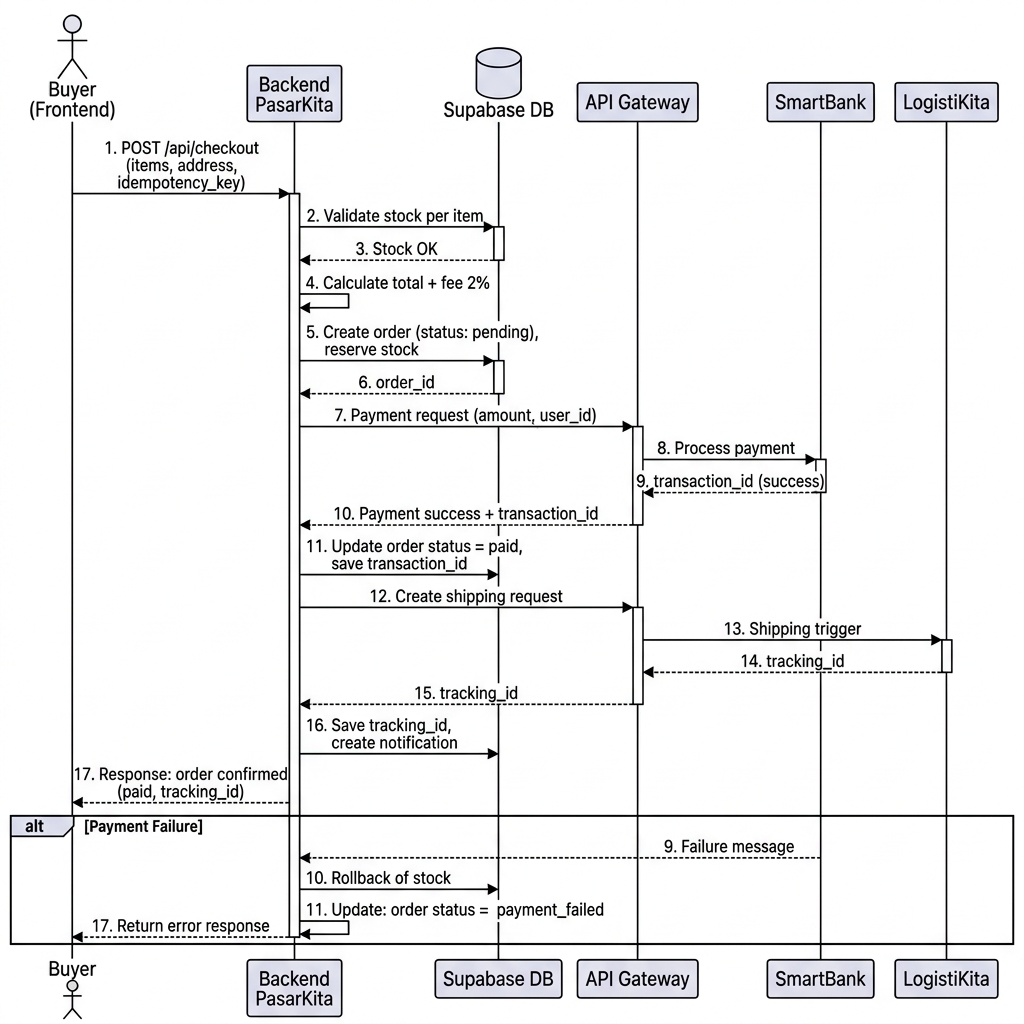
\includegraphics[width=\textwidth]{figures/sequence-checkout.png}
    \caption{Sequence Diagram Alur Checkout PasarKita}
    \label{fig:sequence-checkout}
\end{figure}

Jika pembayaran sukses, \textit{backend} memperbarui \textit{order} ke status
\texttt{paid}, mengirim \textit{trigger} pengiriman ke LogistiKita, menerima
\texttt{tracking\_id}, dan mencatat notifikasi. Jika gagal, stok di-\textit{rollback}
dan \textit{order} diperbarui ke \texttt{payment\_failed}. \textit{Superadmin}
dapat memantau seluruh alur melalui \textit{analytics endpoint} dan
\textit{audit log}.
